\documentclass[beamer]{beamer}
%\documentclass[handout]{beamer}

\usepackage[english]{babel}
\usepackage[utf8]{inputenc}

\newif\ifconference
\newif\ifoneauthor

%\conferencetrue % or
\conferencefalse
\oneauthortrue %or
%\oneauthorfalse

\usepackage[ruled,vlined,linesnumbered]{algorithm2e}
\SetKwRepeat{Do}{do}{while}

\usepackage{tikz}
\usepackage{pdfrender}
\usepackage[absolute,overlay]{textpos}
% ********** to whom **********

\DeclareUnicodeCharacter{00A0}{ }
%eliminar margen
\newcommand\Wider[2][3em]{%
	\makebox[\linewidth][c]{%
		\begin{minipage}{\dimexpr\textwidth+#1\relax}
			\raggedright#2
		\end{minipage}%
	}%
}

\usepackage{beamerthemeshadow}
\usetheme[blackblocktext,nobg,pagenumbers,nocol]{Dresden}

\definecolor{beamer@personal0}{rgb}{0.780,0.780,0.520}
\definecolor{beamer@personal1}{rgb}{0.600,0.600,0.400}
\definecolor{beamer@personal2}{rgb}{0.540,0.540,0.360}
\definecolor{beamer@personal3}{rgb}{0.420,0.420,0.280}
\definecolor{beamer@personal4}{rgb}{0.360,0.360,0.240}
%\definecolor{beamer@personal2}{rgb}{0.600,0.600,0.400}
%\definecolor{beamer@personal1}{rgb}{0.660,0.660,0.440}

\setbeamercolor{block title}{bg=beamer@personal2,fg=white}
\setbeamercolor{block body}{bg=beamer@personal1,fg=white}
\setbeamercolor{block title example}{bg=beamer@personal2,fg=white}
%\setbeamercolor{block body example}{bg=beamer@personal0,fg=black}


\setbeamertemplate{navigation symbols}{}
\setbeamertemplate{blocks}[rounded]% [shadow=false]

\setbeamercolor*{palette secondary}{use=structure,fg=white,bg=beamer@personal1}
\setbeamercolor*{palette tertiary}{use=structure,fg=white,bg=beamer@personal2}

%Amplío el tamaño de los contenidos
\setbeamertemplate{itemize/enumerate body begin}{\large}
\setbeamertemplate{itemize/enumerate subbody begin}{\large}

%en listas
\setbeamercolor{item projected}{bg=beamer@personal1}
\setbeamercolor{subitem projected}{bg=beamer@personal1}

%en figuras
\setbeamercolor{caption name}{fg=beamer@personal2}

%\setbeamertemplate{itemize item}[\color{beamer@personal1}ball]
%\setbeamertemplate{itemize subitem}{\color{beamer@personal1}$\blacktriangleright$}


%Table of contents 
\setbeamerfont{section in toc}{size=\Large}
\setbeamercolor{section in toc}{fg=black}
\setbeamertemplate{sections/subsections in toc}{ \inserttocsectionnumber.~\inserttocsection}

%change margins (latex margins are a little too generous)
\setbeamersize{text margin left=0.75cm,text margin right=1cm} 

%eliminar shadow from titles
\setbeamerfont{frametitle}{size=\LARGE}
\setbeamertemplate{frametitle}{%
	\nointerlineskip%
	\begin{beamercolorbox}[wd=\paperwidth,ht=2.5ex,dp=0.6ex]{frametitle}
		\hspace*{2ex} \insertframetitle %
	\end{beamercolorbox}%
}

\ifoneauthor
\setbeamerfont{author}{size=\fontsize{14}{16}}
\else
\setbeamerfont{author}{size=\fontsize{12}{14}}
\fi
\setbeamerfont{institute}{size=\normalsize\itshape}
\setbeamerfont{title}{size=\fontsize{19}{21}}
\setbeamerfont{subtitle}{size=\Large\normalfont\slshape}

%modificamos pagina de title (dibujo chulo)
\setbeamertemplate{title page}{%
	\begin{tikzpicture}[remember picture,overlay]
	\fill[beamer@personal1]
	([yshift=-5pt]current page.west) rectangle (current page.south east);
	\node[anchor=east] 
	at ([yshift=-70pt]current page.north east) (author)
	{\parbox[t]{.9\paperwidth}{\raggedleft%
			\usebeamerfont{author}\textcolor{beamer@personal2}{%
				\textpdfrender{
					TextRenderingMode=FillStroke,
					FillColor=beamer@personal2,
					LineWidth=.1ex,
				}{\insertauthor}}}};
	\node[anchor=north east] 
	at ([yshift=-80pt]current page.north east) (institute)
	{\parbox[t]{.78\paperwidth}{\raggedleft%
			\usebeamerfont{institute}\textcolor{beamer@personal2}{\insertinstitute}}};
	\node[anchor=south west] 
	at ([yshift=26pt,xshift=15pt]current page.west) (logo)
	{\parbox[t]{.19\paperwidth}{\raggedleft%
			\usebeamercolor[fg]{titlegraphic}\inserttitlegraphic}};
	\node[anchor=east]
	at ([yshift=-50pt,xshift=-20pt]current page.east) (title)
	{\parbox[t]{\textwidth}{\raggedleft%
			\usebeamerfont{title}\textcolor{white}{%
				\textpdfrender{
					TextRenderingMode=FillStroke,
					FillColor=white,
					LineWidth=.1ex,
				}{\inserttitle}}}};
	\node[anchor=east]
	at ([yshift=-80pt,xshift=-20pt]current page.east) (subtitle)
	{\parbox[t]{\paperwidth}{\raggedleft\usebeamerfont{subtitle}\textcolor{white}{\insertsubtitle}}};
	\end{tikzpicture}
}

% different headline
\setbeamertemplate{headline}
{%
	\begin{beamercolorbox}[colsep=0pt]{upper separation line head}
	\end{beamercolorbox}
	\begin{beamercolorbox}{section in head/foot} %
		\vskip2pt\insertnavigation{\paperwidth}\vskip5pt
	\end{beamercolorbox}%
	%\begin{beamercolorbox}[colsep=-0pt]{lower separation line head}
	%\end{beamercolorbox}
}

% different footnote
\setbeamertemplate{footline}
{
	\leavevmode%
	\hbox{
		\begin{beamercolorbox}[wd=1.1\paperwidth,ht=2.25ex,dp=1ex,center]{title in head/foot}%
			\usebeamerfont{title in head/foot}\insertshorttitle
		\end{beamercolorbox}%
	}
}


% logos
\ifconference
\titlegraphic{
\includegraphics[width=2.5cm]{cplex}}
\else
\titlegraphic{
\includegraphics[width=4.5cm]{figuras/cplex}}
\fi
	

\title{Uso de CPLEX junto a Excel}
\subtitle[]{Varias alternativas} 
\author[J.\ Pereira]{Jordi Pereira}
\date[]{5 de enero del 2018}

\institute[UAI]{Faculty of Engineering and Sciences\\
  Universidad Adolfo Ib\'{a}\~{n}ez,\\
  Vi\~{n}a del Mar, Chile}

\begin{document}

	%título
	\begin{frame}[plain]
		\maketitle
	\end{frame}
	
	%table of contents
	\begin{frame}\frametitle{Contenidos}\tableofcontents
	\end{frame} 


\section{Introducción} 
\subsection{}

\frame[t]{ % Broad definition of a packing problem
	\frametitle{Diferentes opciones}
	\vfill
	\begin{itemize}\itemsep2ex
		\item Hay diferentes maneras de asociar Cplex y Excel dependiendo del objetivo buscado.
		\item Veremos aquí varias maneras que van desde la sustitución del Solver de Excel por Cplex hasta referirse a Excel como una fuente de entrada y salida de datos. 
		\item Alguna de las opciones que mostraremos requiere cierto conocimiento de programación
		\item IBM ha ido dejando de ofrecer soporte para alguna de las opciones que veremos (específicamente llamar a Cplex desde Excel).
	\end{itemize}
}

\frame[t]{ % Broad definition of a packing problem
	\frametitle{Modelos}
	A lo largo de los ejemplos veremos dos modelos diferentes que servirán para ilustrar el proceso de modelización y resolución mediante Cplex. Los modelos que veremos son dos problemas clásicos del área:

	\begin{itemize}
		\item Uncapacitated Lot Sizing Problem
		\item Set Covering Problem
	\end{itemize}

	\vfill
	
	Vamos a ver una formulación de cada problema.

}

\frame[t]{ % Broad definition of a packing problem
	\frametitle{Uncapacitated Lot Sizing}
	Modelo estándar de inventarios con demanda determinista y heterogénea en $T$ periodos. 
		
\begin{align*}
\min & ~\sum_{t=1}^{T} c_l y_t + \sum_{t=1}^{T} c_s s_t & \\
\mbox{s.t.} & \\
& x_t + s_{t-1} = d_t + s_t & & 1\leq t \leq T; \\
& x_t \leq \mbox{M} y_t & & 1\leq t\leq T; \\ 
& s_0 = 0 & & \\
& y_t  \in \{0,1\},~x_{t} \geq 0,~s_t \geq 0 & & 1\leq t\leq T.
\end{align*}
	
}

\frame[t]{ % Broad definition of a packing problem
	\frametitle{Set Covering}
	Cubrimiento de conjuntos y subproblema de otros modelos más complejos (itinerarios, localización, \emph{timetabling},...). 
	
	\begin{align*}
	\min & ~\sum_{i=1}^{n} c_i x_i & \\
	\mbox{s.t.} & \\
	& \sum_{i=1}^{n} a_{ij} x_i \geq 1 & & 1\leq j \leq m; \\
	& x_i  \in \{0,1\} & & 1\leq i\leq n.
	\end{align*}
	
}

\section{Cplex+Excel} 
\subsection{}

\frame[t]{ % Introducción CPLEX+excel
	\frametitle{Introducción}
	
	\textbf{Pros:}

		\begin{itemize}\itemsep1ex
		\item A priori, la forma más sencilla de hacer las cosas.
		\item Cplex sustituye a Excel Solver utilizando un interfaz muy similar al del segundo.
		\item Puede incluso llamarse desde una macro.
		\end{itemize}

	\textbf{Contras:}

		\begin{itemize}\itemsep1ex
		\item IBM ya no ofrece soporte para este método (esta opción ya no existe en Cplex 12.7 ni Cplex 12.8, además el módulo dejó de desarrollarse en Excel 2010).
		\item En pocas palabras: \emph{``Use at your own risk"} a sabiendas que tarde o temprano dejará de funcionar según se vayan actualizando los equipos.
		\end{itemize}
}

\frame[t]{ % Cplex
	\frametitle{Activando Cplex en Excel}
	
	Tenemos que activar un módulo en Excel (menú Opciones). 
			\begin{figure}
	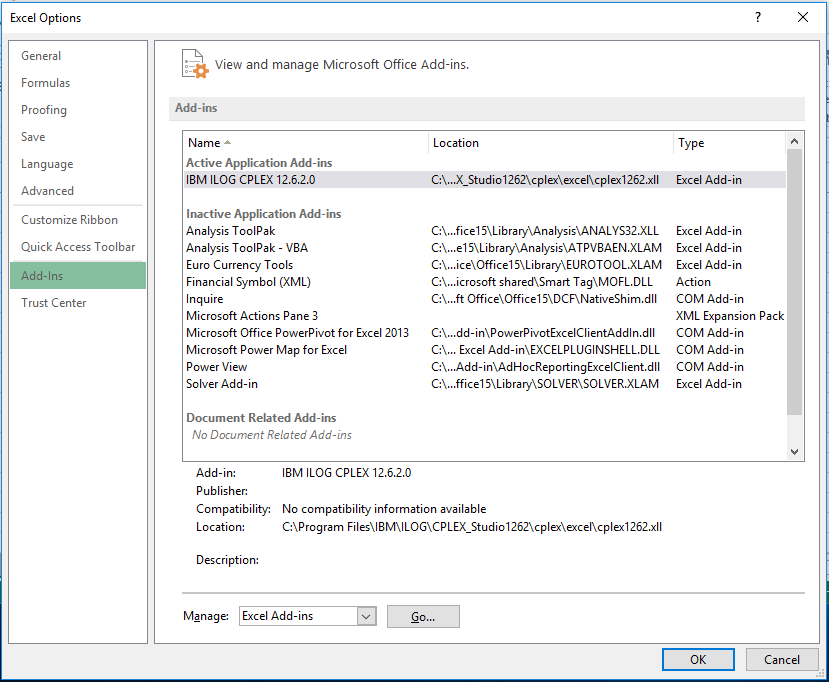
\includegraphics[width=0.7\textwidth]{figuras/corte1}
\end{figure}

}

\frame[t]{ % VBA
	\frametitle{Activando VBA}
	
	Tenemos que mostrar las opciones de desarrollo. 
	\begin{figure}
		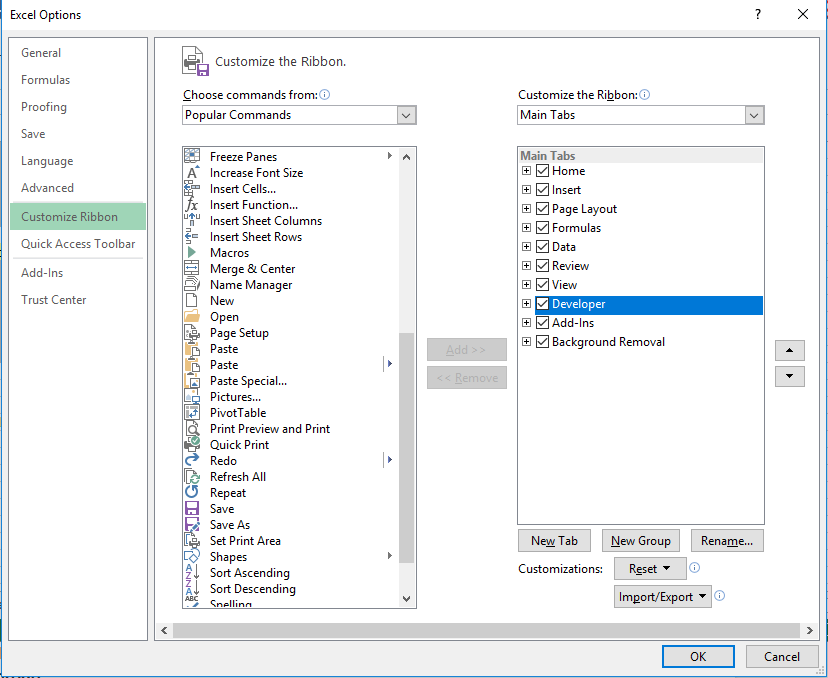
\includegraphics[width=0.7\textwidth]{figuras/corte2}
	\end{figure}
	
}

\frame[t]{ % VBA
	\frametitle{Usar Cplex}
	
	Usar Cplex como sustituto de Solver requiere de los mismos pasos que usaríamos con Solver. 

	\vfill

	\begin{enumerate}
		\item Construir la hoja de cálculo
		\item Determinar las variables (casillas)
		\item Determinar la función objetivo (casilla)
		\item Construir el lado izquierdo y derecho de las restricciones
	\end{enumerate}
	
	\vfill
	
	Puede haber algunos ``problemillas" de uso.
}

\frame[t]{ % Ejemplo 1
	\frametitle{Ejemplo ULS}
	
	\only<1>
	{
		Podemos descargar la hoja de cálculo inicial para hacer el ejercicio de: . 
	}
	\only<2>
	{		
		La versión finalizada puede verse en: 	
	}
	\begin{figure}
	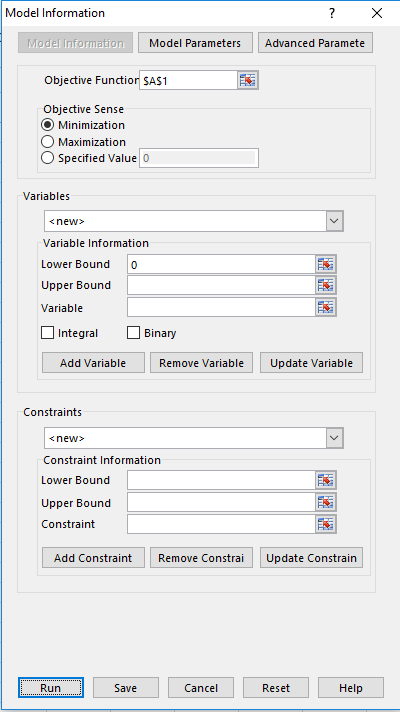
\includegraphics[width=0.30\textwidth]{figuras/corte3}
\end{figure}
	
}

\frame[t]{ % Ejemplo 2
	\frametitle{Ejemplo SCP (versión 1)}
	
	\begin{enumerate}
	\item De forma parecida al caso anterior, podemos resolver el modelo de cubrimiento. Descargar hoja de cálculo de XXX y de XXX para la hoja completa. 
	\item En este caso podemos visualizar que la técnica anterior no escala bien para problemas grandes ni formulaciones en que la matriz $A$ está formada mayoritariamente por entradas iguales 0 (lo que se entiende como una matriz dispersa).
	\item Aquí es cuando se aprecia la oportunidad de mejorar el problema construyendo el modelo de forma programática
	\end{enumerate}
}


\section{OPL+Excel} 
\subsection{}
\frame[t]{ %Truncated enumeration [1]
	\frametitle{BBB}

	Tradicionalmente, las precedencias se relajan y el modelo resultante es una cota inferior.

	\begin{align}
\min &  \sum_{q\in \mathcal{Q}} \bar{c}_{q} z_{q}  & \\
s.t:	&  \sum_{q\in \mathcal{Q}} q_i~ z_{q} =1  & \forall i\in V \\
&  z_{q} \in \{0,1\}  &  \forall q\in Q,k\in K 
\end{align} 
\vfill
Si quisiéramos usar esta formulación para resolver el problema, deberíamos hacer cumplir las precedencias entre asignaciones de forma auxiliar.

}


\section{JuMP+Excel} 
\subsection{}
\frame[t]{ %Truncated enumeration [1]
	\frametitle{CCC}
	
	Tradicionalmente, las precedencias se relajan y el modelo resultante es una cota inferior.
	
	\begin{align}
		\min &  \sum_{q\in \mathcal{Q}} \bar{c}_{q} z_{q}  & \\
		s.t:	&  \sum_{q\in \mathcal{Q}} q_i~ z_{q} =1  & \forall i\in V \\
		&  z_{q} \in \{0,1\}  &  \forall q\in Q,k\in K 
	\end{align} 
	\vfill
	Si quisiéramos usar esta formulación para resolver el problema, deberíamos hacer cumplir las precedencias entre asignaciones de forma auxiliar.
	
}


 
\end{document}
